%
%  Vincent Yannello
%
\documentclass[12pt,fullpage]{article}
\usepackage{fullpage}
\usepackage{psfrag}                                          % LaTeX graphics tool
\usepackage{pslatex}                                         % avoids the default cmr font
\usepackage{graphicx}                                        % graphics package 
\usepackage{epsfig}                                          % figures
\usepackage{hyperref}
\usepackage{color}

\begin{document}

\noindent
{\bf von Mises distribution} (from \color{blue}\url{http://www.math.wm.edu/~leemis/chart/UDR/UDR.html}\color{black})

\noindent
The shorthand $X \sim {\rm von\ Mises}(\kappa, \mu)$ is used to indicate that the
random variable $X$ has the von Mises distribution with shape parameter $\kappa$ and location parameter $\mu$.
A von Mises random variable~$X$ with parameters $\kappa$ and $\mu$ has probability density function 
$$
f(x) = \, {\frac {{e ^ {\kappa \,\cos \left( x - \mu \right) }}}{2 \pi 
\ {\it I_0}  \kern -.08 em \left(\kappa \right) }} \qquad \qquad 0 < x < 2\pi
$$
for all $\kappa$ and for $ 0 < \mu < 2\pi$. The Modified Bessel function of the first kind of order 0
is used for the von Mises random variable and is defined as
$$
I_0 (\kappa) = \displaystyle\sum\limits_{i = 0} ^ {\infty} \frac{\kappa ^ {2i}}{2 ^ {2i} (i !) ^ 2}
$$
for all $\kappa$.
The probability density function for $\mu = \pi$ and two different values of $\kappa$ is illustrated below.
{\begin{figure}[h!]
\begin{center}
\psfrag{lab1}{$\kappa = 1$}
\psfrag{lab2}{$\kappa = 4$}
\psfrag{lab0}{$0$}
\psfrag{labpi}{$\pi$}
\psfrag{lab2pi}{$2\pi$}
\psfrag{labx}{$x$}
\psfrag{labf}{$f(x)$}
\includegraphics[width=3.2in]{VonmisesPlot.ps}
\end{center}
\end{figure}}\\
The cumulative distribution function on
the support of $X$ is
$$
F(x) = P(X \le x) = {\frac {\int _{0} ^ {x} \! {e ^ {\kappa \, \cos \left( t - \mu
 \right) }}{dt}}{2 \pi \ {\it I_0} \kern -.08 em \left(\kappa \right) }} \qquad \qquad 0 < x < 2\pi.
$$
The survivor function, hazard function, inverse distribution function, moment generating function, 
and characteristic functions are all mathematically intractable.
\\
The median of $X$ is
$$
\mu.
$$
The population mean of $X$ is
$$
E[X] = \mu.
$$
The population variance, skewness, and kurtosis of $X$ are mathematically intractable.

\vspace{0.1in}

%\newpage
%\noindent
%{\bf APPL verification:}
%The APPL statements
%\begin{verbatim}
%X := [[x-> exp(kappa*cos(x-mu))/(2*Pi*BesselI(0,kappa))],[0,2*Pi],["Continuous","PDF"]];
%CDF(X);
%SF(X);
%HF(X);
%CHF(X):
%IDF(X);
%Mean(X);
%Variance(X);
%Skewness(X);
%Kurtosis(X);
%MGF(X);
%\end{verbatim}
%verify the cumulative distribution function, survivor function, hazard function, cumulative hazard function, inverse distribution function,  population mean, variance, skewness, kurtosis, and moment generating function.

\end{document}
